\begin{enumerate}
	\item \textbf{Send Vote}
		\begin{enumerate}
			\item \textbf{Service Contract}
				\begin{figure}[H]
					\centering
					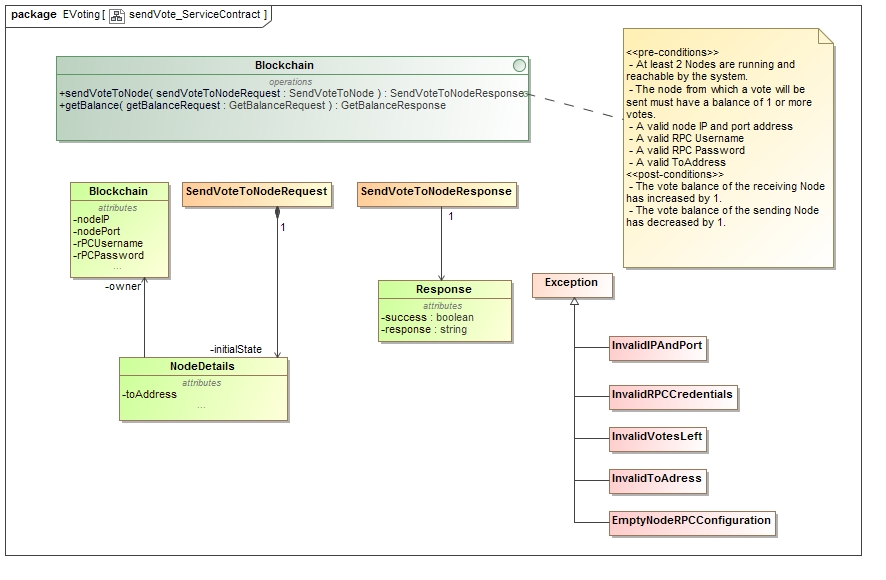
\includegraphics[width=0.75\linewidth]{../Images/Blockchain/ServiceContracts/sendVote_ServiceContract.jpg}
					\caption{Send Vote Service Contract}
				\end{figure}
				
				SendVote requires a ToAddress string which is the receiving node's address. The BlockchainModule is required to be instantiated with a NodeIP string, NodePort string, RPC username string and a RPC password string from where the vote will be sent.
				\newline				
				
				\begin{enumerate}
					\item Pre-conditions
					\begin{itemize}
						\item At least 2 Nodes are running and reachable by the system.
						\item The node from which a vote will be sent must have a balance of at least 1.
						\item A valid node IP and port address.
						\item A valid RPC Username.
						\item A valid RPC Password.
						\item A valid toAddress.
					\end{itemize}
					
					\item Exceptions
					\begin{itemize}
						\item If the configuration strings(node IP address, port address, RPC Username, RPC Password and toAddress) are empty, the EmptyNodeRPCConfiguration exception will be thrown.
						\item If the system cannot reach the node specified by the IP and port address, the InvalidIPAndPort exception will be thrown.
						\item If the specified RPC credentials are incorrect, the InvalidRPCCredentials exception will be thrown.
						\item If toAddress does not exist in the blockchain, the InvalidToAddress exception will be thrown.
						\item If the sending node does not have a balance of at least 1, the InvalidVotesLeft exception will be thrown.
					\end{itemize}
					
					\item Post-conditions
					\begin{itemize}
						\item The vote balance of the receiving node has increased by 1.
						\item The vote balance of the sending node has decreased by 1.
					\end{itemize}
				\end{enumerate}

			
			\item \textbf{Functional Requirements}
				\begin{figure}[H]
					\centering
					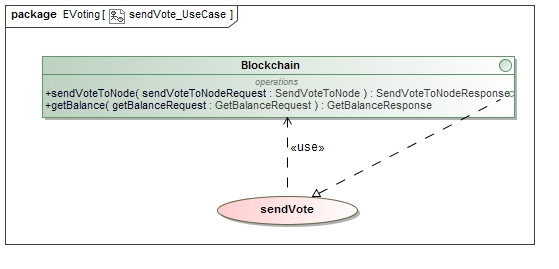
\includegraphics[width=0.75\linewidth]{../Images/Blockchain/UseCase/sendVote_UseCase.jpg}
					\caption{Send Vote Use Case}
				\end{figure}
				The sendVote process does not rely on any other use case, instead the sendVote process will be used by various other use cases.
				\newline
			
			\item \textbf{Process Design}
				\begin{figure}[H]
					\centering
					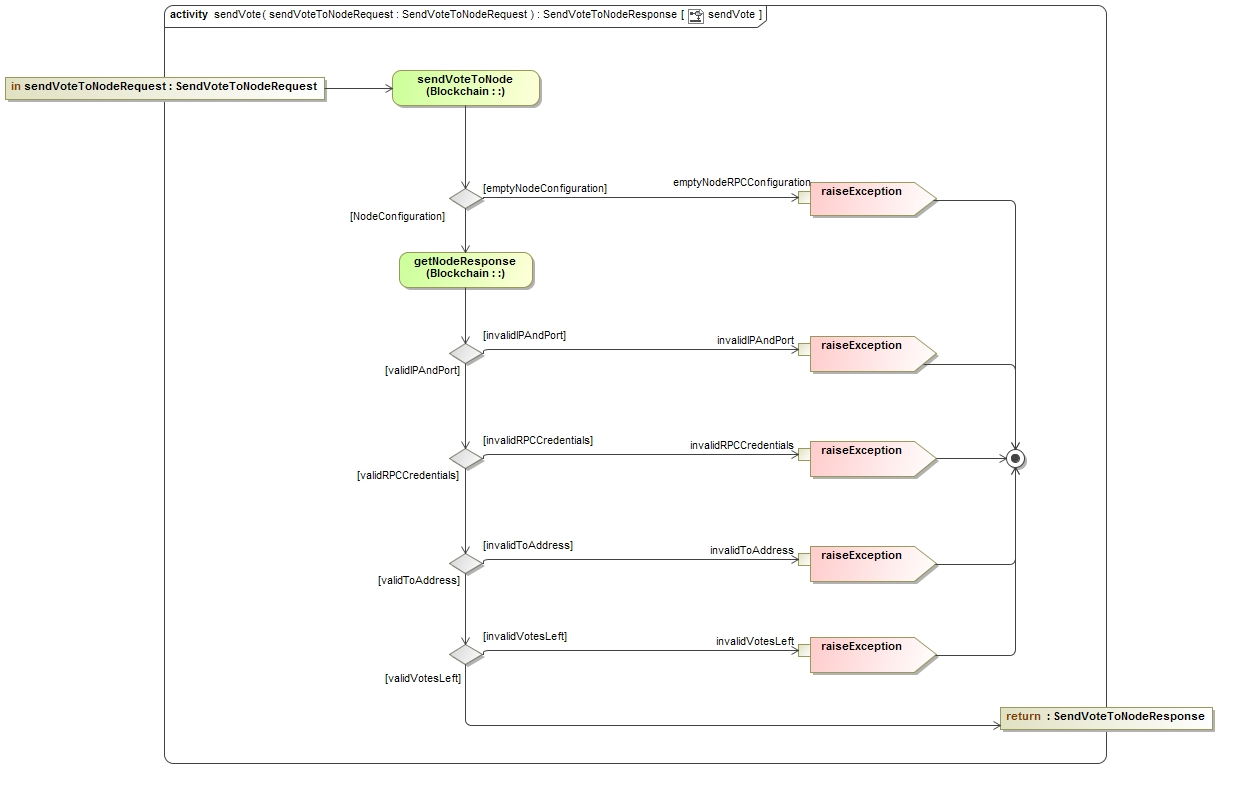
\includegraphics[width=0.75\linewidth]{../Images/Blockchain/Activity/sendVote.jpg}
					\caption{Send Vote Activity}
				\end{figure}
				Once the Send Vote process is called, it first checks if it has all the necesary configuration strings in order to send a vote. If any of these configuration strings are empty, an exception will be thrown. Sencondly the system will check if the node is reachable by sending it a 'ping' request and await a response. If the node does not respond, an exception will be thrown.
				The system will then try to make a transaction in the blockchain from the sending node to the receiving node. If the RPC credentials are incorrect, the InvalidRPCCredentials exception will be thrown. If the ToAddress does not exist in the blockchain, the InvalidToAddress exception will be thrown. If the sending node does not have atleast a balance of 1, the InvalidVotesLeft exception will be thrown. If no exceptions are thrown, and the node returns a string containing the transaction hash, it means the vote has been successfully sent.
				\newline
		\end{enumerate}
	
	\item \textbf{Get Balance}
		\begin{enumerate}
			\item \textbf{Service Contract}
			\begin{figure}[H]
				\centering
				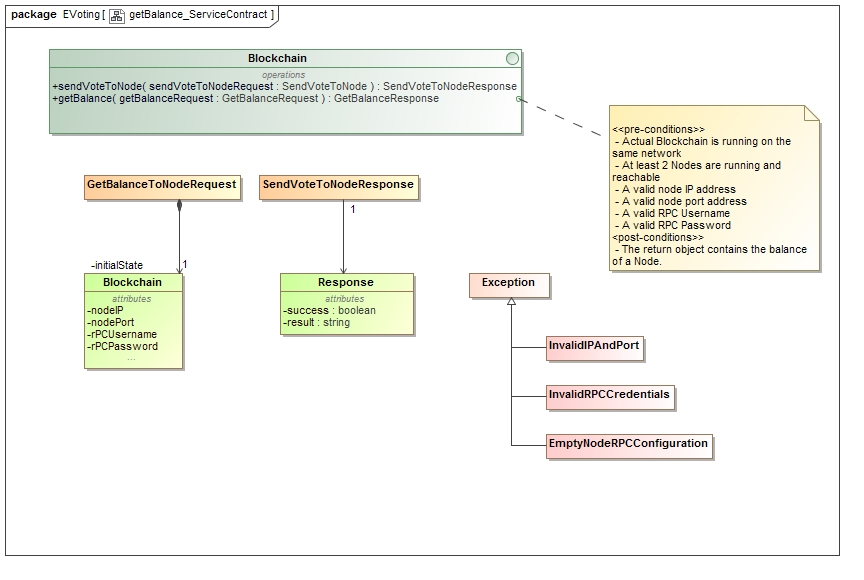
\includegraphics[width=0.75\linewidth]{../Images/Blockchain/ServiceContracts/getBalance_ServiceContract.jpg}
				\caption{Get Balance Service Contract}
			\end{figure}
			 
			In order for a political party to check how many votes they have, the system can return the balance of a specified node. The getBalance process returns the balance of the node specified by the configuration strings (nodeIP and nodePort).
			\newline
			
			\begin{enumerate}
				\item Pre-conditions
				\begin{itemize}
						\item At least 1 Node are running and reachable by the system.
						\item A valid node IP and port address.
						\item A valid RPC Username.
						\item A valid RPC Password.
				\end{itemize}
				
				\item Exceptions
				\begin{itemize}
						\item If the configuration strings(node IP address, port address, RPC Username, RPC Password) are empty, the EmptyNodeRPCConfiguration exception will be thrown.
						\item If the system cannot reach the node specified by the IP and port address, the InvalidIPAndPort exception will be thrown.
						\item If the specified RPC credentials are incorrect, the InvalidRPCCredentials exception will be thrown.
				\end{itemize}
				
				\item Post-conditions
				\begin{itemize}
					\item  The return object contains the balance of a Node in the 'reponse' field.
				\end{itemize}
			\end{enumerate}
			
			\newpage
			
			\item \textbf{Functional Requirements}
			\begin{figure}[H]
				\centering
				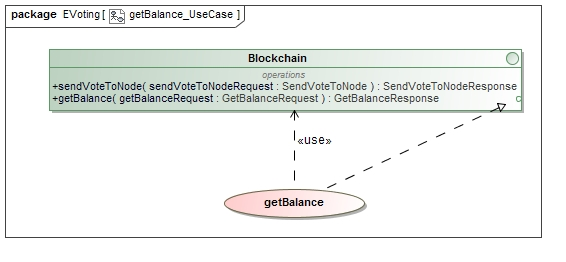
\includegraphics[width=0.75\linewidth]{../Images/Blockchain/UseCase/getBalance_UseCase.jpg}
				\caption{Get Balance Use Case}
			\end{figure}
			
			The getBalance process does not rely on any other use case, instead the Get Balance process will be used by various other use cases.
			\newline
			
			\item \textbf{Process Design}
			\begin{figure}[H]
				\centering
				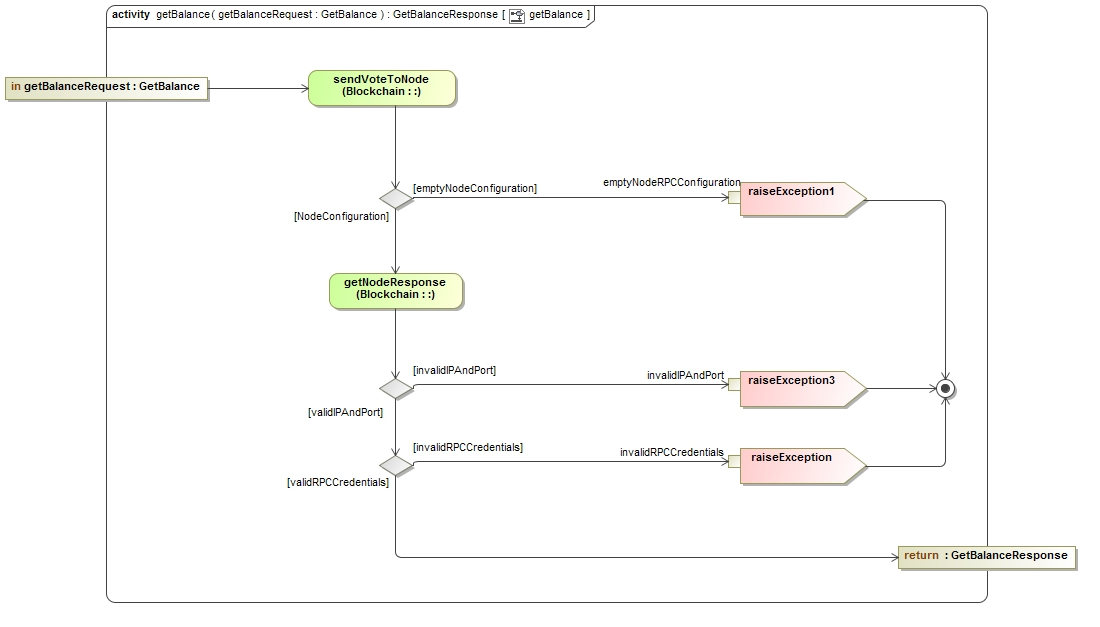
\includegraphics[width=0.75\linewidth]{../Images/Blockchain/Activity/getBalance.jpg}
				\caption{Get Balance Activity}
			\end{figure}
			
				When the getBalance process is called, it first checks if it has all the necesary configuration strings in order to connect to the node. If any of these configuration strings are empty, an exception will be thrown. Sencondly the system will check if the node is reachable by sending it a 'ping' request and await a response. If the node does not respond, an exception will be thrown.
				The system will then try to get the balance of the node. If the RPC credentials are incorrect, the InvalidRPCCredentials exception will be thrown. If no exceptions are thrown, the return object will contain the balance of that node.
			\newline
		\end{enumerate}
\end{enumerate}